%% Copernicus Publications Manuscript Preparation Template for LaTeX Submissions
%% ---------------------------------
%% This template should be used for copernicus.cls
%% The class file and some style files are bundled in the Copernicus Latex Package, which can be downloaded from the different journal webpages.
%% For further assistance please contact Copernicus Publications at: production@copernicus.org
%% https://publications.copernicus.org/for_authors/manuscript_preparation.html


%% Please use the following documentclass and journal abbreviations for discussion papers and final revised papers.

%% 2-column papers and discussion papers
\documentclass[gmd, manuscript]{copernicus}

%% \usepackage commands included in the copernicus.cls:
%\usepackage[german, english]{babel}
%\usepackage{tabularx}
%\usepackage{cancel}
%\usepackage{multirow}
%\usepackage{supertabular}
%\usepackage{algorithmic}
%\usepackage{algorithm}
%\usepackage{amsthm}
%\usepackage{float}
%\usepackage{subfig}
%\usepackage{rotating}


\begin{document}

\title{PRIMAVERA multi climate model analysis at the JASMIN Super Data Cluster}


% \Author[affil]{given_name}{surname}

\Author[1]{Jon}{Seddon}
\Author[2]{Ag}{Stephens}
\Author[1]{Matthew S.}{Mizielinski}

\affil[1]{Met Office Hadley Centre, FitzRoy Road, Exeter, EX1 3PB, UK}
\affil[2]{Centre for Environmental Data Aanalysis, RAL Space, STFC Rutherford Appleton Laboratory, Harwell, Oxford, Didcot, OX11 0QX, UK}

%% The [] brackets identify the author with the corresponding affiliation. 1, 2, 3, etc. should be inserted.



\runningtitle{TEXT}

\runningauthor{TEXT}

\correspondence{Jon Seddon (jon.seddon@metoffice.gov.uk)}



\received{}
\pubdiscuss{} %% only important for two-stage journals
\revised{}
\accepted{}
\published{}

%% These dates will be inserted by Copernicus Publications during the typesetting process.


\firstpage{1}

\maketitle



\begin{abstract}
The PRIMAVERA project aims to develop a new generation of advanced and well-evaluated high-resolution global climate models. As part of PRIMAVERA, seven different climate models were run at a standard and a higher resolution with common initial conditions and forcings to form a multi-model ensemble. The ensemble members were run on high performance computers across Europe. To allow the data from all models to be analysed an approach of taking the analysis to the data was used. All data was transferred to the JASMIN super-data-cluster, where it was catalogued and details made available to users using the PRIMAVERA Data Management Tool's (DMT's) web interface. Users from across the project were able to query the available data using the DMT and then log in to JASMIN to analyse the data. Here we describe how the PRIMAVERA project used JASMIN's facilities to enable users to analyse this multi-model data set. We show how a facility such as JASMIN can be useful for similar multi-institute projects to efficiently share, organise and analyse large volumes of data.
\end{abstract}


\copyrightstatement{Crown Copyright, Met Office}


\introduction  %% \introduction[modified heading if necessary]

The PRIMAVERA project aims to develop a new generation of advanced and well-evaluated high-resolution global climate models. One of PRIMAVERA's core components are the Stream 1 and Stream 2 simulations. These simulations consist of seven different climate models (AWI-CM-1-1, CMCC-CM2, CNRM-CM6-1, EC-Earth3P, ECMWF-IFS, HadGEM3-GC31 and MPI-ESM1-2) being run at their standard resolution (typically  250~km in the atmosphere and 100~km in the ocean) and at a higher resolution (25~km atmosphere and 8-25~km ocean). All models are run with common initial conditions and forcings using the HighResMIP protocol \citep{Haarsma2016}. The simulations were run on high performance computers (HPCs) across Europe. The scientists analysing the model outputs are based at 20 different institutes across Europe with assistance from other global scientists. Because these are global simulations at a high resolution, the total volume of data to be archived is expected to be around 1.6~petabytes (PB).

A Data Management Plan (DMP) was developed to allow this data to be stored, analysed and archived at the JASMIN super-data-cluster. The Data Management Tool (DMT) software was written to implement the DMP.

If JASMIN had not been available for PRIMAVERA to use then it would have been necessary for each of the modelling centres to make their data available, typically on an Earth System Grid Federation (ESGF) node or local FTP server. Anyone wanting to analyse data would need to identify which variables were available and then download them from each modelling centre to their home institute. There would be multiple copies of common datasets and each institute would require significant volumes of storage, transfer bandwidth and compute resources.

\section{JASMIN}

JASMIN is a super-data-cluster that was installed in 2012 \citep{lawrence2013storing}. It is funded by the Natural Environment Research Council (NERC) and the UK Space Agency, and operated by the Science and Technology Facilities Council (STFC). It is located at the STFC Rutherford Appleton Lab, Harwell, UK. JASMIN's Phase 4 update in September 2018 added 38.5~PB of new storage co-located with the existing 4000 cores of compute. The storage and compute are tied together with a low latency network. RAL has a fast connection to JANET, the UK's academic network, which in turn is connected to the G\'{E}ANT European network, allowing fast transfer of data from the HPCs used to run the PRIMAVERA simulations to JASMIN. Additionally, JASMIN is connected to RAL's tape library for the offline storage of data.

The compute at JASMIN is split into interactive data analysis servers, the LOTUS batch processing system and some additional private cloud servers. Part of the storage is dedicated for the Centre for Environmental Data Analysis' (CEDA) archive. The storage for individual projects is split into small chunks called group workspaces (GWS). Each GWS is typically up to 100~terabytes (TB).

All hosts at JASMIN run the Linux operating system and have a suite of modern software tools and programming languages installed for analysing and manipulating common Earth science data formats.

\section{PRIMAVERA}

PRIMAVERA consists of eleven work packages (WPs). The Stream 1 and 2 simulations described here are run and managed by two of the work packages. Several of the other WPs analyse these simulations and compare them with existing simulations, observations and reanalyses. The remaining WPs carry out model development work or run small simulations that don't need to be shared with other WPs. These remaining WPs had a small volume of storage on one of the GWS reserved for them.

The Stream 1 and 2 simulations follow the HighResMIP protocol and will be submitted to the 6th phase of the Coupled Model Intercomparison Project (CMIP6) \citep{Eyring2016}. The Stream 1 simulations consist of a single ensemble member from each model at a standard and a high resolution for six different experiments. The follow on Stream 2 simulations contain additional ensemble members from some of Stream 1 models, but with a reduced data output to minimise the volume of data generated, and some additional simulations to exploit the new physics that has been developed in PRIMAVERA.

While the PRIMAVERA proposal was being developed it was recognized that developing and implementing a data management plan would require a significant number of person months and so resource for these was included in the project proposal.


\section{Data Management Plan}

\begin{figure*}[t]
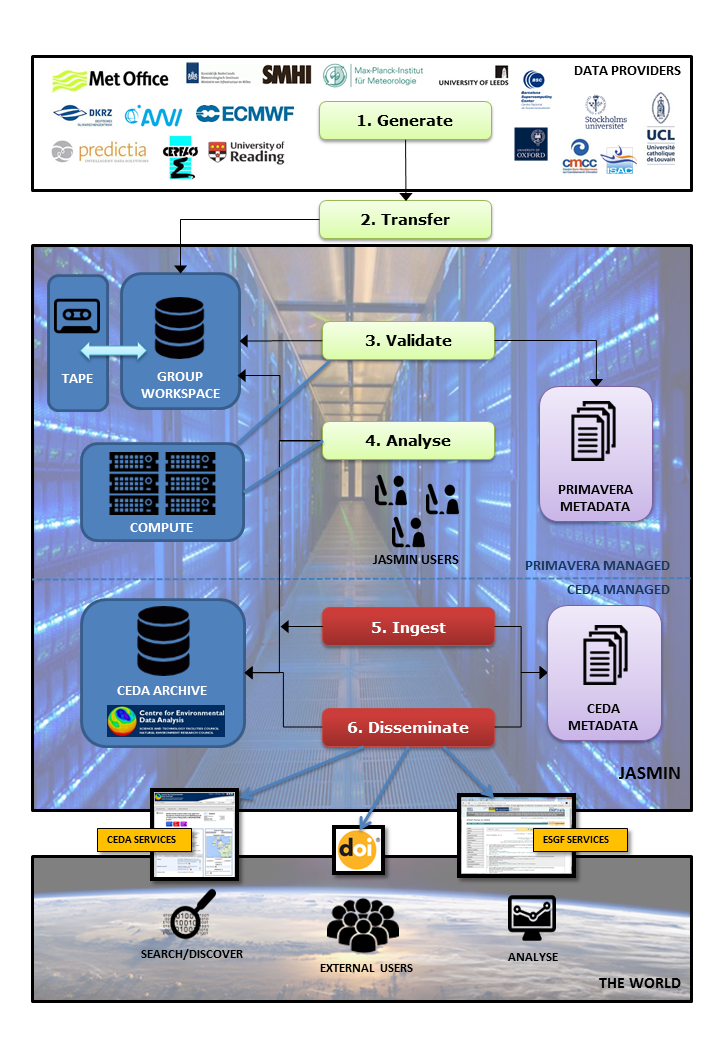
\includegraphics[width=12cm]{fig01.png}
\caption{The workflow developed for PRIMAVERA in the Data Management Plan.}
\label{dmp_workflow}
\end{figure*}

The PRIMAVERA Data Management Plan can be summarised as taking the analysis to the data. Figure~\ref{dmp_workflow} shows the workflow developed in the DMP~\citep{Mizielinski2016}. All data files from the PRIMAVERA simulations will be uploaded to JASMIN. Users are then able to undertake all of their analysis of the data at JASMIN. In previous projects users have downloaded the files that they want to analyse to computing facilities at their home institute. With the volume of data being produced by PRIMAVERA, it is no longer feasible for everyone to take their own copy of the data because the data volumes are too big to store and will take too long to transfer.

Step 1 in the DMP workflow is the generation of data by the modelling centres. The simulations are run on a variety of HPCs across Europe. Each model typically has its own proprietary output file format. It was decided to use the CMIP6 data and metadata standards~\citep{gmd-11-3659-2018} because the data was being submitted to HighResMIP. These standards include using the netCDF format, the file naming structure and the data request. If files had been output by the climate models in a proprietary format then they were post-processed or CMORized (Climate Model Output Rewriter~\citep{Nadeau2019}) into CMIP6 compliant netCDF files. Other models were able to output compliant netCDF files directly.

The second step in the workflow is the transfer of the data from the HPCs or post-processing systems to JASMIN. A discussion on the transfer techniques used and the rates achieved is given in Sect.~\ref{transfer_rates}. The data is uploaded to one of the PRIMAVERA GWS' at JASMIN.

Step 3 in the workflow is the validation of the data. Validation includes checking that the data and metadata standards have been complied with and the extraction of metadata to store in the PRIMAVERA database~\citep{Seddon2020}. Once the validation is complete the files are written to tape and removed from GWS to create space for other uploads. After the upload and validation of the data, in Step 4, users analyse and work with the uploaded data. 

Steps 5 and 6 in the workflow were managed by CEDA rather than the PRIMAVERA project. Uploaded data is ingested into the CEDA archives and is then available for dissemination to the global community using CEDA's ESGF node.


\subsection{JASMIN Resources Allocated}

After reviewing the DMP, PRIMAVERA was allocated 440~TB of storage at JASMIN split across  five group workspaces. A server in the JASMIN internal cloud was allocated, which was given a domain name and  HTTPS access allowed to it from the Internet.

It was originally estimated that around 2.5~PB of data would be generated by the project. Therefore, only a subset data could be held on disk at once. The remaining data would have to be held on tape and moved to GWS when it was required. The DMP describes how the DMT would allow data to be efficiently and reliably moved between tape and GWS and its current location to be tracked.

\subsection{Typical Analysis Workflow}

\begin{figure}[t]
	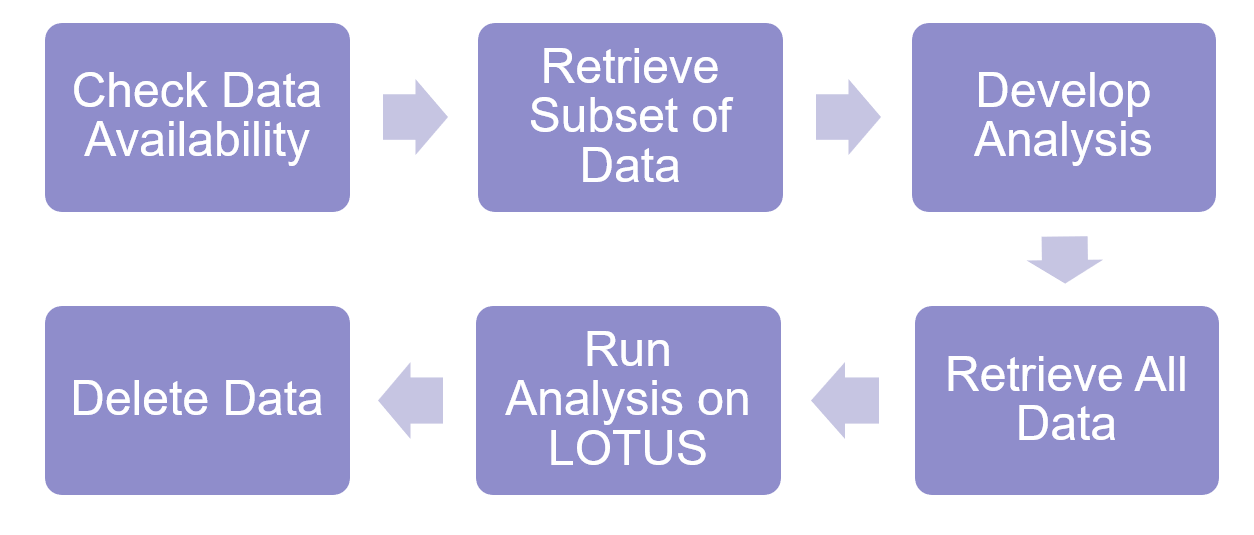
\includegraphics[width=8.3cm]{fig02.png}
	\caption{The workflow required by users working with the PRIMAVERA data at JASMIN.}
	\label{analysis_workflow}
\end{figure}

Figure~\ref{analysis_workflow} shows the workflow that must be adopted by users working with the PRIMAVERA data at JASMIN. Users first use the DMT's web interface to identify what data has been uploaded. If the data they require is not available on disk then they use the DMT's web interface to request that a subset of their data is restored from tape to disk. The DMT sends them an email when their requested data is available on disk and they can then work on JASMIN's interactive servers to develop and test their analysis code. Once this code has been tested and is working they use the DMT to request that all of the data they require is restored from tape to disk. Once the full dataset is available on GWS then the analysis is run on the LOTUS batch processing cluster. Finally, once users are happy with the results of their analysis, they mark the data as finished in the DMT's web interface. The DMT can then delete the data from disk to create space for other users' data.

\section{Data Management Tool}

The DMT was developed to track and control the flow of PRIMAVERA data around JASMIN and to allow users to query what data is available and its location. It consists of a PostgreSQL database and custom software written in the Python programming language, using the Django web framework. The database is installed on a dedicated server, along with web server software and the DMT software. The software was also installed on the JASMIN file system and the server's firewall opened to allow database access from JASMIN's interactive servers, all hosts in the LOTUS cluster and the tape servers. Access to the database from LOTUS allows the validation of uploaded data to be submitted to the batch processing cluster, allowing large uploads to be processed in parallel, which was important for processing steps that take a long time, such as calculating checksums.

\begin{figure}[t]
	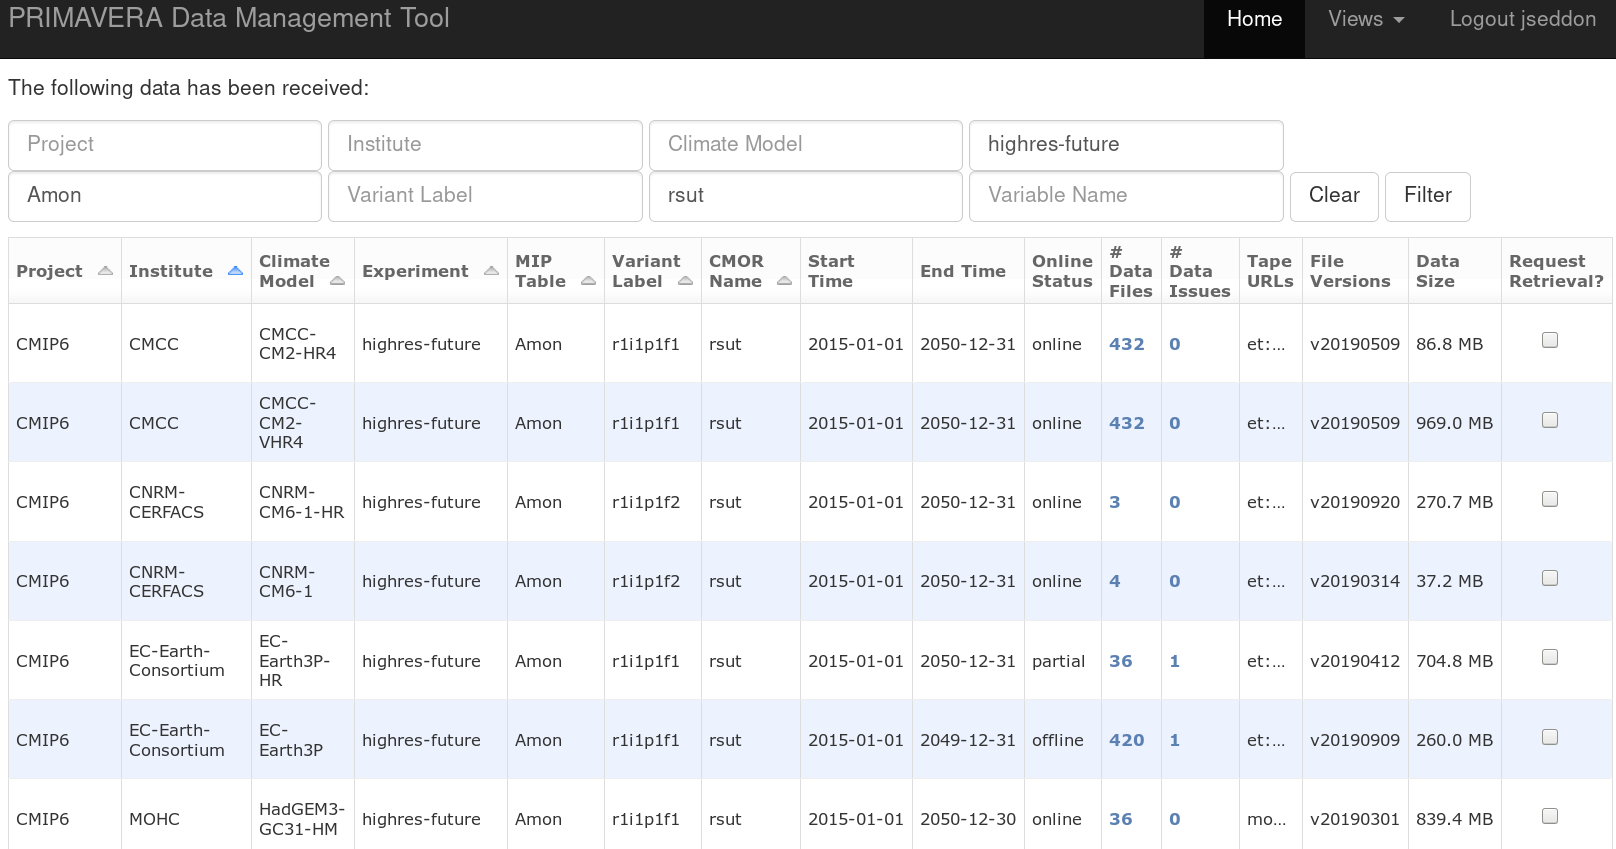
\includegraphics[width=12cm]{fig03.png}
	\caption{The workflow required by users working with the PRIMAVERA data at JASMIN.}
	\label{dmt_query}
\end{figure}

A typical screenshot from a user querying the DMT's web interface is shown in Fig.~\ref{dmt_query}. In this example the variable ``rsut'' the top of atmosphere outgoing shortwave radiation, from the ``highres-future'' coupled future experiment is being queried. A value of ``offline'' in the ``Online Status'' column shows that the files for this simulation are currently only available on tape, a value of ``partial'' shows that some files are on disk, but others are only available on tape and ``online'' shows that all files are available on disk. The ``Request Retrieval?'' column allows users to indicate that they want to work with this variable. If the variable's files need to be restored from tape to disk then this is queued for retrieval and the user is emailed when the data becomes available. The DMT contains a similar page to allow users to view the data that they've requested and allows them to indicate that it has been finished with and can be deleted from disk if required.

The DMT software~\citep{Seddon2019} is distributed under an open source license. Development of the DMT began in April 2016 and the first data was published in the DMT in May 2017, during this period one developer was largely working full time on its development. Development work has continued intermittently since then to improve the flow of data through the system and to allow the publication of data to the ESGF. 


\subsection{DMT Internal Structure}
Internally, the DMT's primary data object is a DataRequest. DataRequest objects consist of a VariableRequest object and details of the institute, climate model, experiment and variant label providing this DataRequest. The VariableRequest objects specify a CMIP6 variable and table along with additional metadata. The VariableRequest objects were created directly from the CMIP6 HighResMIP data request. During the development of the data management plan, a shared spreadsheet was created from the HighResMIP data request and each institute edited the spreadsheet to indicate the variables that they would generate. The DataRequest objects were created programmatically from this spreadsheet. A facility to allow institutes to update the data that they provide during the project is available.

A DataFile object is created for each file uploaded to JASMIN during the validation process. Each DataFile is related to a DataRequest. All views in the DMT's web interface are generated from these DataRequest objects. All objects are Django model objects.

\section{Data Transfer}
\label{transfer_rates}

Table~\ref{rates_achieved} shows the sustained rates achieved when transferring data from the data providers to JASMIN in megabytes per second (MB~s$^{-1}$). JASMIN contains several servers in a data transfer zone, whose connection to the Internet and to JASMIN has been designed for the maximum throughput of data transfers. At the start of the project it had been assumed that parallel transfer protocols such as BBCP or GridFTP would provide the best transfer rates and data providers were encouraged to use these. In reality, most data providers used the techniques that they were most familiar with as long as they gave sufficiently fast transfer rates. The rates achieved depend on many factors including the file system at either end, the load on the server and network at either end and the network between the servers. The best transfer rate from a site was over 200~MB~s$^{-1}$, which is 16.5 TB per day. Typical rates were 30~MB~s$^{-1}$ (2.5 TB per day). These rates were sufficient to complete the project on time. It is hoped that with further optimisation work transfer rates of 5.0~TB per day could be achieved.

The collection of all of PRIMAVERA's data at JASMIN was only possible because of the transfer rates that were achieved. If JASMIN had not been available, then the project would have been dependent upon the transfer rates that could be achieved between many different sites.


\section{Future Opportunities}

\subsection{Platforms}

\subsubsection{JASMIN}
JASMIN has been essential to the success of PRIMAVERA. JASMIN has a finite capacity and so may not be able to support all further projects that would benefit from having access to it. Facilities similar to JASMIN providing additional capacity would be incredibly useful for collaborative projects like PRIMAVERA. Facilities like JASMIN reduce the need for all institutes participating in a project to have their own large data storage and data analysis facilities. Such facilities also reduce the volume of data that needs to be transferred, which is important as such simulations increase in resolution and complexity, and therefore increase in size.

Access to facilities such as JASMIN also allow scientists from developing countries who do not currently have access to high-performance data analysis facilities locally to analyse large data sets. The CP4-Africa~\citep{Stratton2018} convection-permitting regional climate simulations over Africa are now available at JASMIN~\citep{Senior2019} and have been analysed at JASMIN by scientists working from Africa. Tools to access JASMIN-like facilities must be robust to the potentially slow and unreliable Internet connections that may be encountered in developing countries.


\subsubsection{Public Cloud}
Public cloud computing technologies could provide an alternative to a facility such as JASMIN. Users have been using local Unix based computers to analyse data for many years. The change from working locally to working remotely at JASMIN was therefore only a small change for users. The change was assisted by JASMIN's comprehensive documentation and the development of additional documentation and demonstration videos by the PRIMAVERA project. JASMIN's mix of interactive servers and the batch processing cluster allowed for the easy development of analysis software and its running on the full multi-model datasets. Moving users' analyses to the cloud would be a significant change for users, who would require additional assistance with this. However, the use of public cloud technology would allow the compute to be easily scaled to the amount required at any one time, and provide large volumes of data storage and remote access to the data for all users.

Funding for the provision of public cloud computing would need to be resolved. STFC were PRIMAVERA project partners and received some funding for this. Central project funding would be required for all of the storage of data and compute for its analysis in the public cloud. Compute in the public cloud is billed per second. A worst case estimate of the total duration of compute in the project would have to be made in the proposal and funding allocated for this. Data sharing outside of the project could be made easier in a public cloud based solution as external users could fund their own processing costs, whereas in PRIMAVERA they have had to be invited onto the JASMIN platform.

Significant design and development work is required before projects like PRIMAVERA can move their data storage and analysis to the public cloud.

\subsection{Software}

The DMT software worked well for the PRIMAVERA project. It was the first time that such a tool had been developed. The current DMT implementation makes some assumptions about the layout of the storage allocated to PRIMAVERA at JASMIN and about the structure of the PRIMAVERA data. It will require refactoring before it can be used in other projects. The current version of the DMT has shown that such a tool is feasible and can improve the efficiency of data management, discovery and storage in such a project.

New software technologies such as Pangeo offer further benefits if a public cloud solution was used or if external access was available to multiple JASMIN-like facilities around the world~\citep{Pangeo}. Pangeo is a collection of software packages to enable Earth science research in cloud and HPC environments. It allows data to be distributed across different storage areas and schedules processing on the compute attached to each storage. Pangeo could reduce the volume of data needing to be transferred in future projects. Model output data would be uploaded to a cloud location close to the data provider. Just the metadata would be uploaded to a central (or distributed) catalogue. Tools such as Pangeo would then run users' analysis software on the compute where each dataset is stored and only the small volume of analysis results would need to to transferred back to the user.

\conclusions  %% \conclusions[modified heading if necessary]

PRIMAVERA's Data Management Plan and access to the JASMIN super-data-cluster have been essential to the success of the PRIMAVERA project. The DMP and JASMIN have allowed over 100 researchers to collaboratively analyse a multi-model high-resolution set of climate simulations. Over 1.6~PB of data has been collected in a single location where users have been able to analyse the data on interactive data access servers and through a batch processing cluster. The Data Management Tool has reduced the volume of expensive disk storage required by allowing data to be seamlessly moved between tape and disk under the control of data users.

Access to JASMIN has been essential to the success of the PRIMAVERA project. Continued expansion of JASMIN is necessary to allow it to continue supporting such projects. Alternatively, the development of new facilities that provide similar functionality to JASMIN would benefit the Earth sciences community. The use of facilities such as JASMIN and the PRIMAVERA Data Management Tool have proven successful and are recommended for adoption by similar projects.

The tools developed by the PRIMAVERA project have successfully demonstrated the feasibility of such techniques. The tools have been made freely available, but require some development before they can be seamlessly adopted by other projects. The inclusion in the project proposal of dedicated time resource for data management and developing the DMT contributed to the success.

%% The following commands are for the statements about the availability of data sets and/or software code corresponding to the manuscript.
%% It is strongly recommended to make use of these sections in case data sets and/or software code have been part of your research the article is based on.

\codeavailability{The PRIMAVERA Data Management Tool's source code can be found in a publicly available GitHub repository distributed under a BSD 3-Clause license \citep{Seddon2019}. Additional code is similarly available in the validation tool~\citep{Seddon2020} and MIP tables~\citep{Nadeau2018} with similar licenses.}



% \dataavailability{TEXT} %% use this section when having only data sets available


% \codedataavailability{TEXT} %% use this section when having data sets and software code available


% \sampleavailability{TEXT} %% use this section when having geoscientific samples available


% \videosupplement{TEXT} %% use this section when having video supplements available


%\appendix
%\section{}    %% Appendix A
%
%\subsection{}     %% Appendix A1, A2, etc.


\noappendix       %% use this to mark the end of the appendix section

%% Regarding figures and tables in appendices, the following two options are possible depending on your general handling of figures and tables in the manuscript environment:

%% Option 1: If you sorted all figures and tables into the sections of the text, please also sort the appendix figures and appendix tables into the respective appendix sections.
%% They will be correctly named automatically.

%% Option 2: If you put all figures after the reference list, please insert appendix tables and figures after the normal tables and figures.
%% To rename them correctly to A1, A2, etc., please add the following commands in front of them:

\appendixfigures  %% needs to be added in front of appendix figures

\appendixtables   %% needs to be added in front of appendix tables

\begin{table}[t]
	\caption{The rates achieved while transferring data from the data providers to JASMIN.}
	\begin{tabular}{lll}
		\tophline
		Transfer from & Rate achieved & Protocol used \\
		\middlehline
		Toulouse, France & 13~MB~s$^{-1}$ & 4 BBCP jobs in parallel, with 4 streams each \\
		Hamburg, Germany & 20 to 55~MB~s$^{-1}$ & globus-url-copy \\
		Bologna, Italy & 34~MB~s$^{-1}$ average, 69~MB~s$^{-1}$ peak & gridftp, with 4 concurrent FTP connections 8 process in parallel \\
		Bologna (Cineca), Italy & 200 to 300~MB~s$^{-1}$ & 5 parallel \texttt{rsync -av -e "ssh -c arcfour"} \\
		Barcelona, Spain & 13~MB~s$^{-1}$ & rsync \\
		Exeter, UK & 30~MB~s$^{-1}$ & 5 \texttt{moo get} in parallel \\
		Reading, UK & 85~MB~s$^{-1}$ & 4 parallel \texttt{rsync -rvz --rsh="ssh -c arcfour"} \\
		\bottomhline
	\end{tabular}
	\belowtable{} % Table Footnotes
	\label{rates_achieved}
\end{table}


%% Please add \clearpage between each table and/or figure. Further guidelines on figures and tables can be found below.



\authorcontribution{MM and AS developed the PRIMAVERA data management plan. JS and AS then developed and implemented the DMT and managed the data upload and data availability. JS prepared the manuscript with contributions from all co-authors.} %% this section is mandatory for the journals ACP and GMD. For all other journals it is strongly recommended to make use of this section

\competinginterests{The authors declare that they have no conflict of interest.} %% this section is mandatory even if you declare that no competing interests are present

% \disclaimer{TEXT} %% optional section

\begin{acknowledgements}
The PRIMAVERA project is funded by the European Union's Horizon 2020 programme, Grant Agreement no. 641727. This work used JASMIN, the UK's collaborative data analysis environment (http://jasmin.ac.uk). The authors would like to thank all of the STFC staff who design and maintain JASMIN, without whom this work would not have been possible. The data providers from the PRIMAVERA modelling centres should also be thanked for their hard work complying with the metadata standards and their enthusiasm to use the workflows developed in the project, along with all of PRIMAVERA's users.
\end{acknowledgements}




%% REFERENCES

%% The reference list is compiled as follows:

%\begin{thebibliography}{}
%
%\bibitem[AUTHOR(YEAR)]{LABEL1}
%REFERENCE 1
%
%\bibitem[AUTHOR(YEAR)]{LABEL2}
%REFERENCE 2
%
%\end{thebibliography}

%% Since the Copernicus LaTeX package includes the BibTeX style file copernicus.bst,
%% authors experienced with BibTeX only have to include the following two lines:
%%
\bibliographystyle{copernicus}
\bibliography{jasmin-paper.bib}
%%
%% URLs and DOIs can be entered in your BibTeX file as:
%%
%% URL = {http://www.xyz.org/~jones/idx_g.htm}
%% DOI = {10.5194/xyz}


%% LITERATURE CITATIONS
%%
%% command                        & example result
%% \citet{jones90}|               & Jones et al. (1990)
%% \citep{jones90}|               & (Jones et al., 1990)
%% \citep{jones90,jones93}|       & (Jones et al., 1990, 1993)
%% \citep[p.~32]{jones90}|        & (Jones et al., 1990, p.~32)
%% \citep[e.g.,][]{jones90}|      & (e.g., Jones et al., 1990)
%% \citep[e.g.,][p.~32]{jones90}| & (e.g., Jones et al., 1990, p.~32)
%% \citeauthor{jones90}|          & Jones et al.
%% \citeyear{jones90}|            & 1990



%% FIGURES

%% When figures and tables are placed at the end of the MS (article in one-column style), please add \clearpage
%% between bibliography and first table and/or figure as well as between each table and/or figure.


%% ONE-COLUMN FIGURES

%%f
%\begin{figure}[t]
%\includegraphics[width=8.3cm]{FILE NAME}
%\caption{TEXT}
%\end{figure}
%
%%% TWO-COLUMN FIGURES
%
%%f
%\begin{figure*}[t]
%\includegraphics[width=12cm]{FILE NAME}
%\caption{TEXT}
%\end{figure*}
%
%
%%% TABLES
%%%
%%% The different columns must be separated with a & command and should
%%% end with \\ to identify the column brake.
%
%%% ONE-COLUMN TABLE
%
%%t
%\begin{table}[t]
%\caption{TEXT}
%\begin{tabular}{column = lcr}
%\tophline
%
%\middlehline
%
%\bottomhline
%\end{tabular}
%\belowtable{} % Table Footnotes
%\end{table}
%
%%% TWO-COLUMN TABLE
%
%%t
%\begin{table*}[t]
%\caption{TEXT}
%\begin{tabular}{column = lcr}
%\tophline
%
%\middlehline
%
%\bottomhline
%\end{tabular}
%\belowtable{} % Table Footnotes
%\end{table*}
%
%%% LANDSCAPE TABLE
%
%%t
%\begin{sidewaystable*}[t]
%\caption{TEXT}
%\begin{tabular}{column = lcr}
%\tophline
%
%\middlehline
%
%\bottomhline
%\end{tabular}
%\belowtable{} % Table Footnotes
%\end{sidewaystable*}
%
%
%%% MATHEMATICAL EXPRESSIONS
%
%%% All papers typeset by Copernicus Publications follow the math typesetting regulations
%%% given by the IUPAC Green Book (IUPAC: Quantities, Units and Symbols in Physical Chemistry,
%%% 2nd Edn., Blackwell Science, available at: http://old.iupac.org/publications/books/gbook/green_book_2ed.pdf, 1993).
%%%
%%% Physical quantities/variables are typeset in italic font (t for time, T for Temperature)
%%% Indices which are not defined are typeset in italic font (x, y, z, a, b, c)
%%% Items/objects which are defined are typeset in roman font (Car A, Car B)
%%% Descriptions/specifications which are defined by itself are typeset in roman font (abs, rel, ref, tot, net, ice)
%%% Abbreviations from 2 letters are typeset in roman font (RH, LAI)
%%% Vectors are identified in bold italic font using \vec{x}
%%% Matrices are identified in bold roman font
%%% Multiplication signs are typeset using the LaTeX commands \times (for vector products, grids, and exponential notations) or \cdot
%%% The character * should not be applied as multiplication sign
%
%
%%% EQUATIONS
%
%%% Single-row equation
%
%\begin{equation}
%
%\end{equation}
%
%%% Multiline equation
%
%\begin{align}
%& 3 + 5 = 8\\
%& 3 + 5 = 8\\
%& 3 + 5 = 8
%\end{align}
%
%
%%% MATRICES
%
%\begin{matrix}
%x & y & z\\
%x & y & z\\
%x & y & z\\
%\end{matrix}
%
%
%%% ALGORITHM
%
%\begin{algorithm}
%\caption{...}
%\label{a1}
%\begin{algorithmic}
%...
%\end{algorithmic}
%\end{algorithm}
%
%
%%% CHEMICAL FORMULAS AND REACTIONS
%
%%% For formulas embedded in the text, please use \chem{}
%
%%% The reaction environment creates labels including the letter R, i.e. (R1), (R2), etc.
%
%\begin{reaction}
%%% \rightarrow should be used for normal (one-way) chemical reactions
%%% \rightleftharpoons should be used for equilibria
%%% \leftrightarrow should be used for resonance structures
%\end{reaction}
%
%
%%% PHYSICAL UNITS
%%%
%%% Please use \unit{} and apply the exponential notation


\end{document}
